\documentclass[twocolumn]{paper}
\usepackage{comment}
\usepackage{authblk}
\usepackage{graphicx}
\usepackage{wrapfig}
\usepackage{cite}
\usepackage{relsize}
\usepackage[margin=1.0in]{geometry}

\title{Blowship - Untraceable Instantaneous Message Transfer via a Central Server}
\author[*]{John Carlyle}
\author[**]{Morgan McDermott}
\affil[*]{University of angry bees}
\affil[**]{University of flightless dragons}

\begin{document}
\maketitle

\section*{Abstract} 
Many systems have been developed that preserve the anonymity of the sender and receiver of data. These systems are typically decentralized, routing messages through some series of trusted or untrusted peers and servers. 

In this paper we present a centralized anonymity system that uses a single, untrusted central server, adapting decentralized p2p protocols to work in this context, and combine these with Computational Private Information Retrieval (CPIR) to enable low-latency, low-overhead anonymous communication. The primary reason behind a centeral server is to have a browser based service which needs a server to initialze the peer to peer network.

\section{Introduction}

Traditional cryptography obsucres the message being sent from one party to another. This is useful for many purposes but there is an important aspect of your communication that is freely availble to anyone observing the transfer: who the message is being sent to. Much work has been done to build networks that can obscure message passing by esentially mixing the messages around in a large group of peers in such a way that a peer in the network, or even a large group of peers cannot figure out where the message is going to end up. Many of these system rely upon the fact that the user is accessing a constantly avaible resource, such as with tor\cite{tor}, or in the case of email one can wait as long as nessesary for a message to be read by the user on the other end.

we are presenting to the reader is Untraceable Instantaneous Messaging, via a central server. Our system of message passing is initiated by the browser, allowing a person to browse to one central location and conveneintly use this service. The central server is primarily used as an entrypoint into a network of peers. The peers are used to obsfucate who is sending messages to whom, allowing the clients to communicate with both private content, all in as close to real time as possible given the constraints of the algorithms being used.


\section{Previous Work}
\begin{description}
\item[Mixes] Mixes are servers through which encrypted messages are sent, hiding the correlation between incoming and outgoing messages using encryption, pooling incoming messages, and a variety of other strategies. Mixes have seen wide use since Chaum first introduced them in his 1981 paper \cite{chaum-mix}. They have been used in systems such as MixMinion\cite{minion-design} to anonymously send and receive email. Onion routing systems such as Tor \cite{tor-design} use series of mixes as proxies for web data. 

\item[Nym systems] Pseudonymous message delivery systems enable users to send and receive messages with a \textit{nym} (pseudonym) that cannot be traced back to their true identity. Many of these systems rely on having an anonymous ``forward'' channel that allows a user to send a message without attackers being able to deduce the recipient - which is what we are attempting to develop in this paper. 

\item[Private Information Retrieval] PIR has been used to facilitate anonymous communication in a variety of ways. The Pynchon Gate \cite{wpes2005} is a nym system that uses information-theoretic PIR as a layer of indirection between a user and their nym - allowing users to retrieve mail sent to their nym with information-theoretic privacy guarantees. Tor-PIR \cite{TODO} uses PIR to distribute information about servers without forcing users to download the entire directory. 

\end{description}

\section{Measuring Anonymity}
  \textit{Anonymity sets}, introduced by Chaum in his Dining Cryptographers paper \cite{chaum-dc}, are widely used to analyze the anonymity provided by various p2p privacy schemes. Given a message and whatever information an attacker has obtained, the anonymity set for that message is the set of users who could have sent it. An anonymity set of size 1 means that the attacker knows exactly who sent the message.

This measure fails to capture some of the information gathered by the attacker. If, for instance, certain members of an anonymity set are more likely to have sent the message (which is never the case in Chaum's DC networks \cite{chaum-dc}), this information is not captured by the size of the anonymity set. 

To solve this problem, Diaz \cite{Diaz02} and Serjantov \cite{Serj02} independently developed almost identical solutions. Their idea is this: given a message, consider the probability distribution of its senders. The entropy of this probability distribution then represents the number of bits an attacker still needs to obtain in order to identify the sender of the message. 

Serjantov \cite{Serj02} calls this measure the \textit{size} $S$ of the anonymity probability distribution. Given $U$ is the set of all users, and $p_u$ is the probability that $u \in U$ sent the message under its probability distribution for users, then the $size$ of the probability distribution is:

\begin{center}
$ S = - \mathlarger{\sum}\limits_{u \in U} p_u $log$_2(p_u)$
\end{center}

For example, if we give one user a probability $1$ of sending the message, all other users have probability 0, and $S = -(1 * 0) = 0$, meaning the attacker needs no more information to identify the user. 



\section{Privacy Goals}
  The goal of this system is to provide a method for communicating securely between parties through a central server with low latency and low communication overhead. We attempt to satisfy these requirements assuming the intermediate server may be compromised. By communicating securely we mean specifically (using terminology from \textbf{[6]}):
  \\\\\textbf{Communication Privacy}. Any party Eve cannot read the contents of intercepted messages sent between any two parties Alice and Bob. 
  \\\textbf{Participant Privacy}. This is also called \textbf{Unobservability} and \textbf{Untraceability}. Any party Eve cannot determine with probability $p > \epsilon$ that Alice and Bob are communicating, given any chosen $\epsilon$ (with a clear lower bound of $\epsilon > 1/N$ where $N$ is the number of participants). The ability of multiple participants to collude and determine this with $p > \epsilon$ must be well defined.
  \\\textbf{Destination Privacy}. Any party Eve in the network cannot determine the final destination of any party Alice's messages. This is a less stringent requirement than Participant Privacy.
\section{Central Server Communication}
 The majority of research into anonymous communication uses decentralized p2p networks. In some cases, however, it is necessary (and possibly beneficial) to communicate through a central server. Many of the developed p2p techniques can be adapted by using a pseudo-p2p protocol, by having peers communicate with each other indirectly through the central server. 

 In p2p protocols, delivering a message via a chain of peers or servers is a standard method to achieve anonymity. In this system we'll use terminology from Tor and call the chain of peers a message passes through a $circuit$. A pseudo-p2p circuit then consists of an alternating chain of peer-server and server-peer communications.

\begin{figure}[ht]
  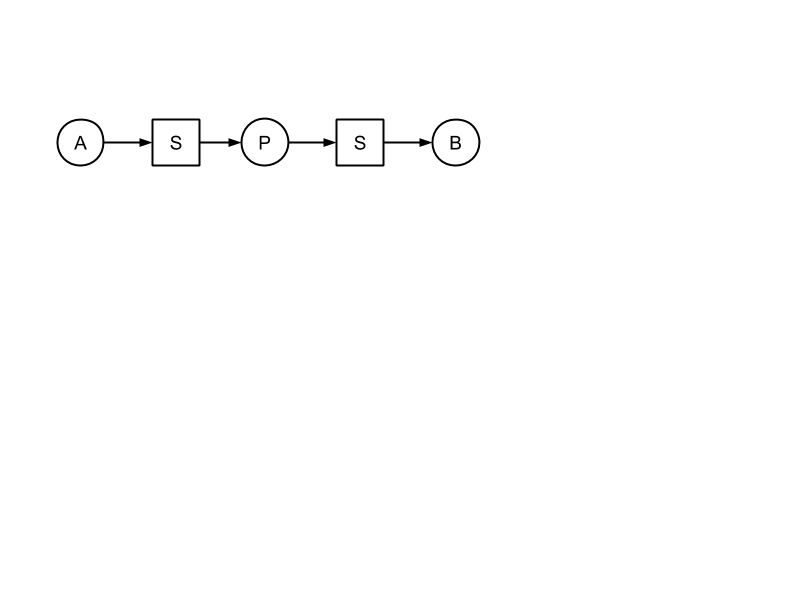
\includegraphics[width=230px]{PSP.png}
  \caption{A simple pseudo-p2p circuit}
\end{figure}

\subsection{Basic Protocol}
Assume that Alice has obtained Bob's public key and unique ID while maintaining her anonymity. Assume also that Alice can obtain the public keys and IDs for $n \le N$ peers at random while hiding her choice from Surge. 

Alice can then send a message to bob that will follow the path $A \rightarrow P_1 \rightarrow S \rightarrow ... \rightarrow S \rightarrow P_n \rightarrow B$ by sending the following message to Surge: 
\\
Let $M = E_{KRA}[  time || nonce || message ]$
\\Let $F_{ij}[x] = E_{KUi}[ ID_j || E_{KUj}[ x ] ]$
\\
Alice sends: $F_{S1}[F_{S2}[...F_{nB}[ M ]]]$ to Surge. 

Each successive party receives a message and an ID to forward that message to, and only that party can read its message. Importantly, any Penguin or Proletariat without collusion from Surge doesn't gain any information about the source or destination of the message it's passing along. 

Note that Surge can't track a message by its contents, since it gets decrypted and changed by each successive peer. 

In this system, peers operate exactly as MIXes in the literature \cite{chaum-mix} . That is, they prevent traffic correlation by removing a layer of encryption, prevent relay attacks [[[soething]]], as well (as we will discuss) by reordering and batching messages. 
\subsection{Adversaries}
In this context, we have several distinct types of adversaries we must consider:
\begin{enumerate}
  \item\textbf{Penguin.} Penguin is any Peer who can intercept and alter messages being passed through it. 
  \item\textbf{Surge.} Surge is a compromised central Server. He can alter and intercept any messages passing through, and can provide bogus information to any peer.
  \item\textbf{Proletariat.} The Proletariat is a group of colluding Penguins.
  \item\textbf{The Palace.} The Palace is a collusion of the Proletariat and Surge.
\end{enumerate}
\subsection{Security Flaws}
Here we'll perform a simplified analysis of the security flaws of the basic, naive system described so far. 
Let $P_{AB}$ be the probability that Alice sent a given message that was delivered to to Bob. 
\begin{enumerate}
\item\textbf{Linear Chain.} If we assume that Alice's message is the only message sent by any of $P_1 ... P_n$, $Surge$ can determine that $P_{AB} > (n+1)^{-1} \gg 1/N$. This is because Surge knows that one of $A \cup \{P_1 ... P_n\}$ talked to Bob.
\item\textbf{Collusion.} If  $s$ peers collude with Surge to form the Palace, then the Palace can determine on average (depending on which peers Alice picked), that $P_{AB} > (n/(N-s)+1)^{-1}$ - that is, Alice has a chance $1 - (N-s)/N$ of each peer being compromised and not contributing to her privacy.
\item\textbf{Timing.} Even if $P_1 ... P_n$ are sending other messages, if Surge knows the probability distribution of the peer delay between receiving a message and forwarding it, he can discover the increased probability that Alice and Bob are talking. 
\item\textbf{Multiple Communications.} If Alice sends another message to Bob, or Bob back to Alice, the chance that they are communicating increases even more. 
\item\textbf{Man in the Middle.} If Alice acquries Bob's public key from Surge (and vice-versa), there's nothing to stop Surge from mounting a Man in the Middle attack given this simple model. 
\end{enumerate}
This is fairly poor security. If Alice chooses $n = 5$, then if her chosen peers send no other messages until hers is delivered, Surge knows $P_{AB} > 1/6$ chance that Alice is talking to Bob. If $60\%$ of peers are part of the Palace, then Surge possibly knows $P_{AB} = 1$ if $n \subset s$, but the expectation is $E[P_{AB}] = 1/3$.

\subsection{Solutions}
To begin solving these problems, change the protocol so that any non-Penguin peer will always wait until it can send two or more messages simultaneously. This is equivilant to turning each peer into a 2-Threshold mix. \cite{TODO}

If we assume that there is not a Palace, then Alice needs only choose $n = log(N)$, If every node sends 2 messages at once, and her message passes through $log(N)$ nodes, then there are $2^n = N$ possible messages that Alice sent, and hopefully $N$ possible destinations. The likelihood is that in $log(N)$ steps from Alice, there will be less than $2^n$ unique recipients of messages, but we can adjust for this by increasing the number of nodes $n$ we choose. If every node has an average unique branching factor of $z$ rather than $2$, we can just set $n = log_z(N)$ and then $z^{log_z(N)} = 1/N$. Then, the $size$ of Alice's anonymity probability distribution is $\approx 1$ since the sender probabilities are roughly uniform.

In this way Surge gains no information about the sender of the message. If Surge knows Alice will choose $n = log(N)$, then he can rule out any peer in the chain with distance $< n$ from Alice, and then $P_{AB} = 2^{-(log(N)-1)} = 2/N$, and $S = - \frac{1}{4} log(\frac{1}{2N})$ which is still reasonable, though Alice could compensate by randomly choosing the length of her circuit. 

\subsection{The Palace} Assuming the set $S$ peers colludes with the server where $s = |S| > n$, and Alice chooses her circuit $C$ of peers randomly (where $|C| = n$), there is unfortunately some chance that $R \subset S$ and so $P_{AB} = 1$. If $s = \phi*N$ peers are part of the palace, on average $E[P_{AB}] = 2^{-\phi log(N)}$. The chance Surge can tell with probability $> \gamma$ that Alice and Bob are talking to eachother, $p(P_{AB} > \gamma)$ requires Alice choosing $x$ Palace members as peers. 

This happens with probability $\sum\limits_{i=x}^n\phi^i$ where 
\\ $P_{AB} = 2^{-(n - x)} = 2^{-(log(N) - x)} = \gamma$
\\ $x = 2^{loglog(N)/\gamma}$

\begin{figure}[ht]
    \begin{tabular}{| l | l | l | l | l | l |}
      \hline
      $\phi$ & N & $E[P_{AB}]$ & x & n & $p(P_{AB} > 0.5)$ \\\hline
      0.5 & 1000 & 0.031 & 4 & 10 & 0.12\\
      0.5 & 10000 & 0.01 & 4 & 14 & 0.12\\
      0.5 & 100000 & 0.003 & 5 & 17 & 0.06\\
      \hline
    \end{tabular}
    \caption{Table 42.42 - Probabilities things are bad}
\end{figure}

While less than ideal this is not bad. The chance that Surge, having $50\%$ of peers colluding with him, can tell that Alice is talking to Bob with probability $> 0.5$ is only $12\%$. 

\begin{comment}
TODO: Apply PIR to obtain security guarantees even when $R \subset S$
\end{comment}

\subsection{Peer Discovery and MITM brainstorming}

Lying about who's online - If you want to send a message to a real node ``B'' but B is not listed as online, you won't send a message. However, if he lists ``B'' as online, ``B'' can be used to route messages validly by everyone. 

Chain verification - Keep a web of trust with the length of the path to a person inversely proportional to how trusted they are. Share web of trust with those we communicate with - only share nodes with a certain level of trust, and then trust nodes discovered this way with diminished trust. 

If initial trust is only spread through person to person contact, then assigning negative trust is valuable because it reduces the value of colluding human nodes. 

* Have nodes sign messages as they pass through, so that the path can be tested/verified. 

\subsection{Peer Discovery}
Unfortunately, if peers discover eachother through Surge, he can ensure that any peer only knows about compromised peers (Effectively making $\phi = 1$).

This is a common problem in Onion routing schemes like Tor, as well as Mix networks. If directory servers collude with some routing servers, they can choose to only broadcast the existence of the compromised routing servers.

MixMinion \cite{minion-design} solves these problems by having a small group of directory servers that only update nightly, having servers sign each other's directories, and ensuring that users download entire directories. These solutions are not feasible in our case since the set of online users is constantly in flux, and is likely to be too large to be sent to every user. Tor \cite{tor-design} likewise has a small number of trusted directory servers that share infrequently updated, signed directories.



\subsection{Man in the Middle.} If both Alice and Bob are online, then they could use Diffie Hellman to ensure that Surge isn't acting as a Man in the middle. However, we'd like to allow offline delivery of messages.

This requires some form of web of trust, or some means of verifying public keys without trusting Surge. 

Users should maintain a list of known keys to make stuff good. 

\subsection{Peers as Mixes}
As previously discussed, peers act as mixes in this system - inheriting both their benefits and vulnerabilities. Many types of mixes have been developed, and Serjantov \cite{trickle02} has compiled common attacks and solutions. 
A mix holds on to incoming messages until its \textbf{flush function} is satisfied, then it forwards some subset of its collected messages. Common attacks are variants of the $n - 1$ or $flooding$ attack, in which an attacker fills the mix with its own fake messages and then sends the 1 message he wishes to track. 

All known mix types are vulnerable to such exact attacks \cite{trickle02} -  attacks that allow an attacker to know whether his attack was successful or not and try again if not. Since in our threat model Surge has complete access to the message history of each peer as well as the ability to delay and insert as many messages as he desires, trying to prevent these attacks by implementing a better flush function is even more futile. 

Fortunately, due to the nature of this system we can provide almost complete protection with \textbf{cover traffic} \cite{trickle02}, or having each peer send dummy messages along with the messages it's forwarding. A peer will at minimum send one dummy message along with every real message, maintaining a branching factor greater than two at every hop. Typically providing complete protection with cover traffic is difficult - it requires the mix to choose dummy message recipients uniformally from all users. In our system, however, randomly and anonymously choosing other online peers is designed to be efficient.

It would also be possible to use inter-mix detours\cite{TODO}, having peers randomly decide to introduce new hops to prevent Surge from recognizing his own messages sent during an $n - 1$ attack. However, this reduces reliability, increases latency, and given the protection that cover traffic provides seems unnecessary in this system. 

\section{Applying PIR}
An obvious way to utilize PIR for anonymous communication is as a ``Dead Drop''. If we have a PIR server Charlie, Alice could write her messages to block $i$ in Charlie's PIR database, then bob could request block $i$ anonymously. This could enable us to increase the size of Alice's anonymity set (retaining a uniform distribution of probabilities, as well) while reducing our circuit length significantly. 

There are several problems with this configuration, however.

First, Alice must communicate Charlie's ID and $i$ to bob anonymously. This could happen via the pseudo-p2p protocol as above. 

Second, Alice and Bob both start talking to Charlie around the same time. If Charlie suspects Alice and Bob are talking to eachother, he can easily create a fake PIR database for all of Alice's inserts and all of Bob's retrievals, and if they continue to communicate normally he has found a connection. 


\section{Future Work}
\begin{description}
  \item[Pseudonymity.] Allow for parties to communicate securely without knowing eachother's identities. Currently our system relys heavily (at least when a person first enters the network) on the fact that the person initiating the communication knows the person's key with whom he wants to communciate.

  \item[Faster circuits.] Like Tor, we could use layers of symmetric encryption between successive pairs of peers in a circuit. Using a public/symmetric system like Tor could help with pseudonymity as well. Currently we are doing a lot of public/private key encryption which is slow.

  \item[DoS.] We would like to address the issue of DoS attacks against networks by requiring messages to be accompanied by a proof of work. This would allow us to require that the messages being sent are by computers that are also helping to suport the network.
\end{description}

\newpage

\bibliography{paper.bib}
\bibliographystyle{plain}
\end{document}
